\chapter{Week8}
\section{Friday}\index{week8_Thursday_lecture}
This lecture will discuss the multi-variable calculus. 
\subsection{Introduction to metric space}
The multi-variable calculus aims to study the function $f:\mathbb{R}^m\mapsto\mathbb{R}^n$:
%. To begin with, let's assume $n=1$, i.e., 
\[
f(\underbrace{x_1,x_2,\dots,x_m}_{\bm x})=(f_1(\bm x),f_2(\bm x),\dots,f_n(\bm x))
\]
To begin with, let's assume $n=1$, i.e., we study only one component in RHS first. The preliminaries for this concept are limit points or something else. Let's define them in high dimension first.
\paragraph{Generalization from $\mathbb{R}$ to $\mathbb{R}^2$}The distance between two points in $\mathbb{R}^2$ is usually defined as follows:
\[
\begin{array}{l}
\bm x=(x_1,x_2)\\
\bm y=(y_1,y_2)
\end{array}\implies
d(\bm x,\bm y)=\sqrt{(x_1-y_1)^2+(x_2-y_2)^2}\quad\mbox{($L_2$ norm)}
\]
\begin{itemize}
\item
Sometimes another distance measrue is $d_1(\bm x,\bm y)=|x_1-y_1|+|x_2-y_2|$, which is called $L_1$ norm
\item
Or more generally, $d_{\infty}(\bm x,\bm y)=\max_{1\le i\le n}|x_i-y_i|$, which is called $L_{\infty}$ norm.
\end{itemize}
Those distance measures are essentially the same in order, i.e.,
\begin{align*}
\frac{1}{\sqrt{2}}d(\bm x,\bm y)&\le d_1(\bm x,\bm y)\le\sqrt{2}d(\bm x,\bm y),\qquad \forall x,y\in\mathbb{R}^2\\
d(\bm x,\bm y)&\le d_{\infty}(\bm x,\bm y)\le\sqrt{2}d(\bm x,\bm y),\qquad \forall x,y\in\mathbb{R}^2
\end{align*}
\begin{remark}
\begin{itemize}
\item
For those distance measures with the same order, the corresponding properties defined with those measures are also nearly the same. We always define the $L_2$ norm as our distance measure by default.
\item
However, one distance measure is different in order from those above: 
\[
\bar{d}(\bm x,\bm y)=\left\{
\begin{aligned}
1,&\quad\mbox{if }x\ne y\\
0,&\quad\mbox{otherwise}
\end{aligned}
\right.
\]
\end{itemize}
\end{remark}
\begin{definition}[Matric Space]
The binary operation $d:\mathcal{H}\times\mathcal{H}\mapsto\mathbb{R}$ is called a matric if the following are satisfied:
\begin{enumerate}
\item
$d(\bm x,\bm y)\ge0$,$\forall x,y\in\mathcal{H}$;
\item
$d(\bm x,\bm y)=d(\bm y,\bm x)$,$\forall x,y\in\mathcal{H}$;
\item
$d(\bm x,\bm z)\le d(\bm x,\bm y)+d(\bm y,\bm z)$, $\forall x,y,z\in\mathcal{H}$,
\end{enumerate}
where $\mathcal{H}$ is called the \emph{metric space}, e.g., $\mathbb{R}^m$ is a common metric space.
\end{definition}
The reason for defining matric is to describe \emph{convergence} in high dimensions. Let's define the corresponding definitions related to convergence again:
\begin{definition}[Open ball]
The open ball is a set $B_r(\bm a)$ such that
\begin{equation}
B_r(\bm a):=\{\bm x\in\mathcal{H}\mid d(\bm x,\bm a)<r\}
\end{equation}
\end{definition}
Some illustrations for $B_1(\bm0)$ in the metric space $\mathbb{R}^2$ is shown as follows:

\begin{figure} 
  \centering 
  \subfigure[The $L_1$ metric with unit ball $B_1(\bm0)$]{ 
    \label{fig:subfig:a} %% label for first subfigure 
    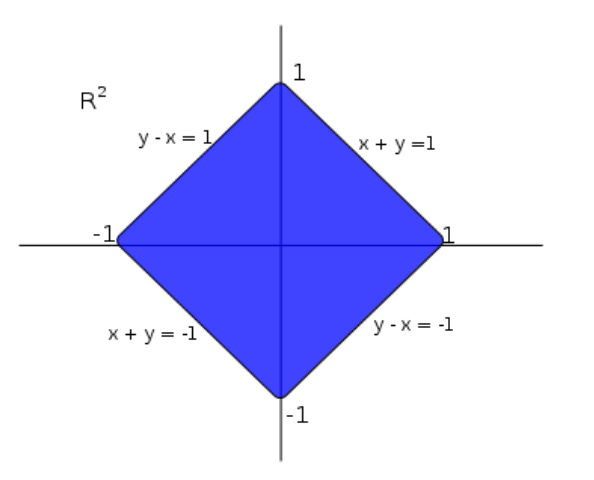
\includegraphics[width=2in]{week8/f_8_1}} 
  \hspace{1in} 
  \subfigure[The $L_2$ metric with unit ball $B_1(\bm0)$]{ 
    \label{fig:subfig:b} %% label for second subfigure 
    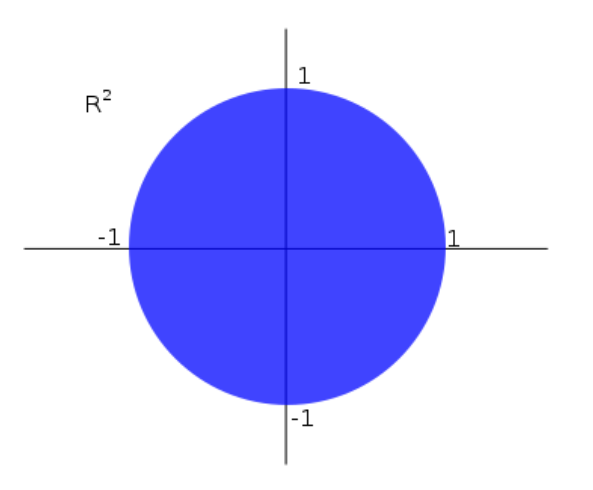
\includegraphics[width=2in]{week8/f_8_2}} 
  \label{fig:subfig} %% label for entire figure 
    \subfigure[The $L_\infty$ metric with unit ball $B_1(\bm0)$]{ 
    \label{fig:subfig:b} %% label for second subfigure 
    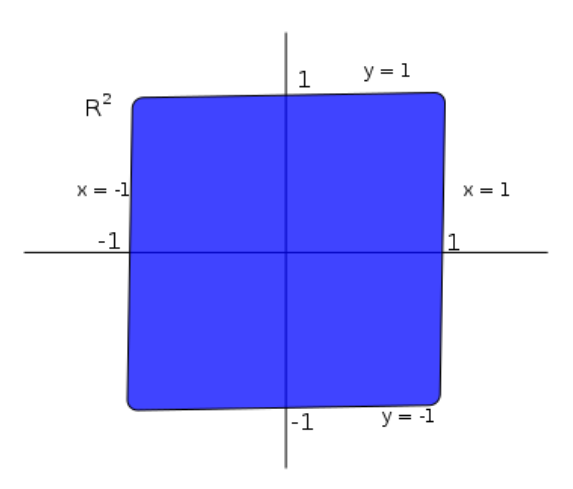
\includegraphics[width=2in]{week8/f_8_3}} 
  \caption{illustrations for $B_1(\bm0)$ in the metric space $\mathbb{R}^2$} 
\end{figure}
\begin{definition}[Convergence]
The sequence defined on the metric space $(\mathcal{H},d)$ is convergent to $x_0$ if $d(x_n,x_0)\to0$ as $n\to\infty$, which is denoted as $\lim_{n\to\infty}x_n=x_0$, or simply $x_n\to x_0$
\end{definition}
Check rudin's book in page 32 for the concepts about Openness, closedness, neighborhood, boundness, \emph{compactness}, limit points, \emph{connectness}. In particular, let's discuss something important.
\begin{definition}[Compact]
A set $K$ is said to be compact ifs every open cover has a finite subcover.
\end{definition}
The proof of the proposition that $K$ is compact if it is bounded and closed is left as exercise.
\begin{definition}
A set $S$ is \emph{pathwise} connected if for any two points $\bm x,\bm y\in S$, there exists a `'\emph{path}
`' $\Gamma$ connecting $\bm x$ and $\bm y$, where $\Gamma$ is a continuous function $[0,1]\mapsto S$ with the property that $\Gamma(0)=\bm x,\Gamma(1)=\bm y$. 
\end{definition}
\begin{definition}[Domain]
A domian is an open set which is \emph{path-wise connected}.
\end{definition}
\begin{remark}
An open set is not necessarily path-wise connected.
\end{remark}
\begin{definition}[Oscillation]
\begin{enumerate}
\item
The \emph{oscillation} of $f:X\subseteq\mathbb{R}^m\mapsto\mathbb{R}$ on a set $E\subseteq X$ is $\omega(f;E)=d(f(E))$, where $d$ denote the diameter of the set $f(E)$, i.e.,
\[
\omega(f;E)=d(f(E))=\sup_{x,y\in E}d(f(x),f(y)).
\]
\item
The \emph{oscillation} of $f$ at a point $\bm a$ is
\[
w(f;\bm a)=\lim_{r\to0+}\omega(f;B_{r}(\bm a))
\]
\end{enumerate}
\end{definition}
\paragraph{Local Properties}
\begin{proposition}[Useful Properties]
Let $f$ be a function mapping a metric space $\mathcal{H}$ to $\mathbb{R}^m$, then
\begin{enumerate}
\item
$f$ is continuous at the point $\bm a$ iff $\omega(f;\bm a)=0$
\item
If $f$ is continuous at $\bm a$ with $f(\bm a)>0$, then $f>0$ in some neighborhood of $\bm a$
\item
The linear combinations of continuous functions $(\alpha f+\beta g)$, component-wise products $(f\cdot g)$, or component-wise quotients $(\frac{f}{g},g_i\ne0)$ are also continuous functions
\end{enumerate}
\end{proposition}
\begin{proposition}[Global Properties]
\begin{enumerate}
\item
Let $f:K\mapsto\mathbb{R}^n$ be a continuous function with $K$ being compact, then we have
\begin{enumerate}
\item
$f$ is \emph{uniformly continuous} on $K$
\item
$f$ is \emph{bounded} on $K$
\item
$f$ assumes its maximum and minimum on $K$
\end{enumerate}
\item
Intermediate Value property: If $f:E\mapsto\mathbb{R}$ is continuous, where $E$ is \emph{path-wise connected}, then $f(a)=A$ and $f(b)=B$ implies for all $c$ between $A$ and $B$, there exists $c\in E$ such that $f(c)=C$.
\end{enumerate}
\end{proposition}
\begin{example}
\begin{enumerate}
\item
\[
f(x,y)=\left\{
\begin{aligned}
\frac{xy}{x^2+y^2},&\quad (x,y)\ne(0,0)\\
0,&\quad (x,y)=(0,0)
\end{aligned}
\right.
\]
For any $(x,y)$ on the line $y=mx$, we have
\[
f(x,mx)=\frac{mx^2}{x^2+m^2x^2}=\frac{m}{1+m^2},
\]
thus $\lim_{(x,y)\to(0,0)}f(x,y)$ does not exist sicne different paths toward the origin may lead to a different limit. There is another interesting fact:
\[
\left\{
\begin{aligned}
\lim_{x\to0}\lim_{y\to0}f(x,y)&=0,\\
\lim_{y\to0}\lim_{x\to0}f(x,y)&=0
\end{aligned}
\right.
\]
\item
\[
f(x,y)=\left\{
\begin{aligned}
x+y\sin\frac{1}{x},&x\ne0\\
0,&x=0
\end{aligned}
\right.
\]
Apply $\varepsilon$-$\delta$ language to verify that $\lim_{(x,y)\to(0,0)}f(x,y)=0$, but
\[
\left\{
\begin{aligned}
\lim_{x\to0}\lim_{y\to0}f(x,y)&=0\\
\lim_{y\to0}\lim_{x\to0}f(x,y)&\mbox{ does not exist}
\end{aligned}
\right.
\]
\begin{remark}
The continuity of a function at $x=a$ does not necessaily imply the interchangeability of limit processes. However, the uniform convergence can enable us to arrive at positive results.
\end{remark}

\item
\[
f(x,y)=\left\{
\begin{aligned}
\frac{x^2y}{x^4+y^2},&\quad (x,y)\ne(0,0)\\
0,&\quad (x,y)=(0,0)
\end{aligned}
\right.
\]
For any $(x,y)$ on the line $y=mx$, we have
\[
f(x,mx)=\frac{mx^2\cdot x}{x^4+m^2x^2}=\frac{mx}{x^2+m^2}\to0,\mbox{ as }x\to0
\]
However, for any $(x,y)$ on the line $y=x^2$, we have
\[
f(x,x^2)=\frac{x^2\cdot x^2}{x^4+x^4}=\frac{1}{2},
\]
which means $f$ is not continuous at $(0,0)$.
\item
\[
f(x,y)=\left\{
\begin{aligned}
\frac{x^2y}{x^6+y^2},&\quad (x,y)\ne(0,0)\\
0,&\quad (x,y)=(0,0)
\end{aligned}
\right.
\]
When $y=mx$, we have $f(x,mx)=\frac{mx}{x^4+m^2}\to0$.

When $y=x^3$, we have $f(x,x^3)=\frac{1}{2x}\to\infty$, i.e., $f$ is unbounded near origin.
\end{enumerate}
\end{example}

\paragraph{Question} 
Is it possible that a sphere $S^2$ and a circle $S^1$ are situated such that the distance from any point on the sphere to any point on the circle is the same, i.e., is it possible for a function
\[
d(x,y):S^2\times S^1\mapsto\mathbb{R}
\]
remains constant? When will this fact be possible in $\mathbb{R}^k$?


















